% Source: graduate-coursework/Prior_Semesters/Sp24/EMCH354/assignments/HW3/HW3.tex

\documentclass[border=4pt]{standalone}
\usepackage{amsmath}
\usepackage{courier}
\usepackage{graphicx}
\usepackage{tikz}
\usepackage{xcolor}
\usetikzlibrary{patterns}
\usetikzlibrary{arrows.meta, decorations.pathmorphing}

\definecolor{bluecolor}{RGB}{173,216,230}
\definecolor{purplecolor}{RGB}{210,180,222}
\definecolor{pinkcolor}{RGB}{255,182,193}
\definecolor{orangecolor}{RGB}{252, 213, 180}

\begin{document}
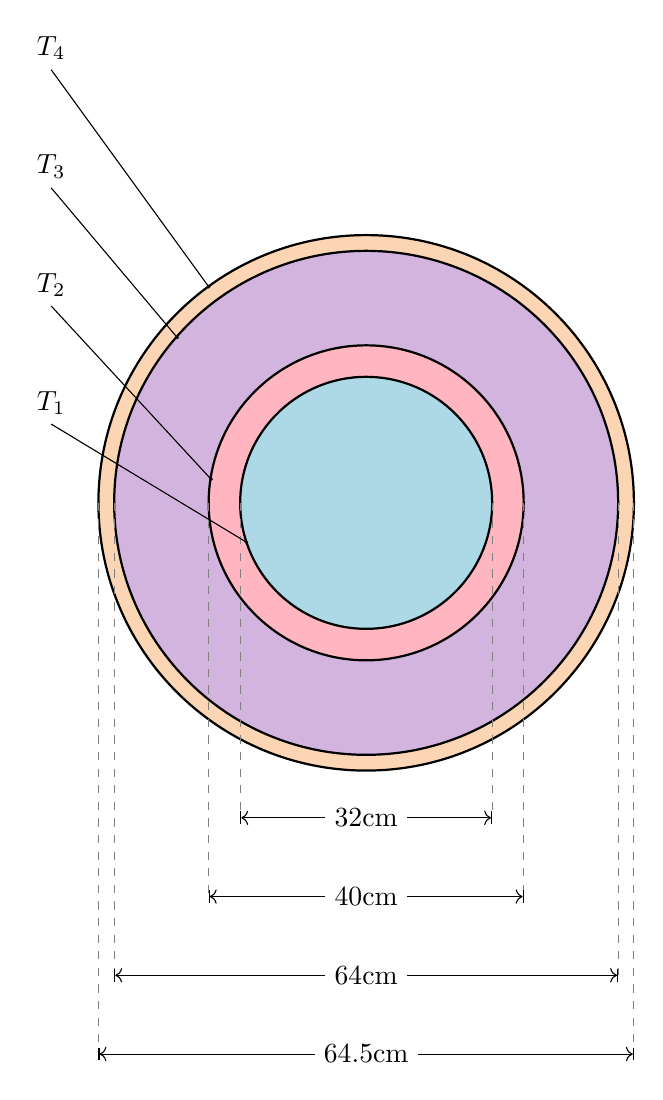
\begin{tikzpicture}[scale=0.1] % Scale down for the diagram to fit in the document.

    % Adding a grid for reference (adjust range and step as needed)
   % \draw[step=5.0, gray, very thin] (-100, -100) grid (100, 100); % Grid lines every 10 units

    % Outermost circle (exaggerated size for visibility)
    \draw[fill=orangecolor, thick] (0,0) circle (34cm); % 68cm diameter
    % Second circle
    \draw[fill=purplecolor, thick] (0,0) circle (32cm); % 64cm diameter
    % Third circle
    \draw[fill=pinkcolor, thick] (0,0) circle (20cm); % 40cm diameter
    % Innermost circle
    \draw[fill=bluecolor, thick] (0,0) circle (16cm); % 32cm diameter
    
    % Vertical guide lines for each circle
    \draw[dashed, gray] (34,0) -- (34,-70); % To edge of outermost circle
    \draw[dashed, gray] (-34,0) -- (-34,-70); % From outermost dimension line to edge
    \draw[dashed, gray] (-32,0) -- (-32,-60); % To edge of second circle
    \draw[dashed, gray] (32,0) -- (32,-60); % From third circle dimension line to edge
    \draw[dashed, gray] (20,0) -- (20,-50); % To edge of innermost circle
    \draw[dashed, gray] (-20,0) -- (-20,-50); % From innermost dimension line to edge
    \draw[dashed, gray] (16,0) -- (16,-40); % To edge of innermost circle
    \draw[dashed, gray] (-16,0) -- (-16,-40); % From innermost dimension line to edge
    
    % Dimensions
    % For outermost circle
    \draw[|<->|] (-34,-70) -- (34,-70) node[midway, fill=white] {64.5cm};
    % For second circle
    \draw[|<->|] (-32,-60) -- (32,-60) node[midway, fill=white] {64cm};
    % For third circle
    \draw[|<->|] (-20,-50) -- (20,-50) node[midway, fill=white] {40cm};
    % For innermost circle
    \draw[|<->|] (-16,-40) -- (16,-40) node[midway, fill=white] {32cm};

    % Line that starts with a small circle and ends with text
    \draw[] (-20,27.45) -- node[at start, circle, fill, inner sep=0.5pt] {} node[at end, above] {$T_4$} (-40, 55);
    \draw[] (-24,21) -- node[at start, circle, fill, inner sep=0.5pt] {} node[at end, above] {$T_3$} (-40, 40);
    \draw[] (-19.7,3) -- node[at start, circle, fill, inner sep=0.5pt] {} node[at end, above] {$T_2$} (-40, 25);
    \draw[] (-15.2,-5) -- node[at start, circle, fill, inner sep=0.5pt] {} node[at end, above] {$T_1$} (-40, 10);

\end{tikzpicture}
\end{document}
